\begin{adjustbox}{width=\textwidth}
	\begin{tikzpicture}[every node/.style={inner sep=0,outer sep=0}]
	
		\node [anchor=north east] (imgDeflektometrie) at (-0.03\textwidth,0) {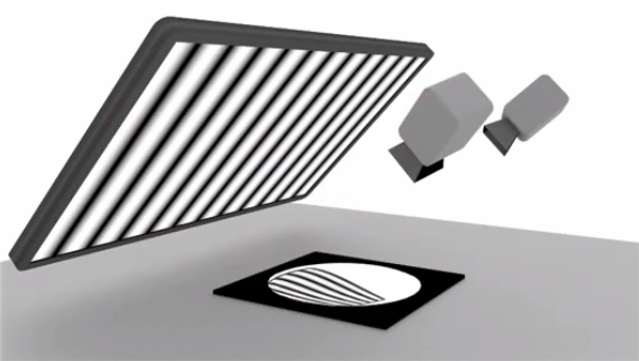
\includegraphics[width=.47\textwidth]{02_grundlagenDerDeflektometrie/spiegelndeOberflaechen/figures/deflektometrie}};
		\node [below=0.2cm of imgDeflektometrie, align=center] {Deflektometrische Verfahren für \\ spiegelnde Oberflächen};
		\node [anchor=north west] (imgProjektion) at (0.03\textwidth,0) {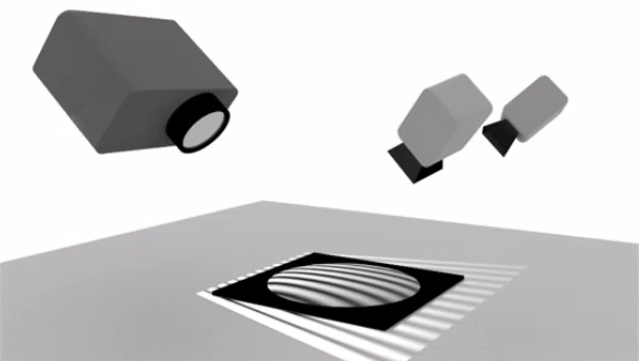
\includegraphics[width=.47\textwidth]{02_grundlagenDerDeflektometrie/spiegelndeOberflaechen/figures/streifenlichtprojektion}};
		\node [below=0.2cm of imgProjektion, align=center] {Streifenlichtprojektion für \\ matte Oberflächen};
		
	\end{tikzpicture}
\end{adjustbox}
\caption[Darstellung der Szenen für spiegelnde und matte Oberflächen]{Darstellung der Szenen für spiegelnde Oberflächen direkt über einen Bildschirm (Deflektometrie) und für matte Oberflächen über einen Projektor (Streifenlichtprojektion). \cite{jenaerOK}}